%%%%%%%%%%%%%%%%%%%%%%%% ExtendedAbstract.tex %%%%%%%%%%%%%%%%%%%%%%%%
%                                                                    %
%  Template for the 10-page extended abstract to be submitted for    %
%  the MSc degree conferral at Instituto Superior Tecnico.           %
%                                                                    %
%  Author:                                                           %
%                                                                    %
%       Andre C. Marta                                               %
%       Area Cientifica de Mecanica Aplicada e Aeroespacial          %
%       Departamento de Engenharia Mecanica                          %
%       Instituto Superior Tecnico                                   %
%       Av. Rovisco Pais                                             %
%       1049-001 Lisboa                                              %
%       Portugal                                                     %
%       Tel: +351 21 841 9466                                        %
%                        3466 (extension)                            %
%       Email: andre.marta@ist.utl.pt                                %
%                                                                    %
%  Created:       Dec  2, 2011                                       %
%  Last Modified: Dec 27, 2011                                       %
%%%%%%%%%%%%%%%%%%%%%%%%%%%%%%%%%%%%%%%%%%%%%%%%%%%%%%%%%%%%%%%%%%%%%%
% This document uses the LaTeX class file "article.cls"              %
%%%%%%%%%%%%%%%%%%%%%%%%%%%%%%%%%%%%%%%%%%%%%%%%%%%%%%%%%%%%%%%%%%%%%%
\documentclass[10pt,a4paper,twocolumn]{article} % Changed from 8pt to 10pt, since it is the minimum allowed by the template, i.e., it doesn't compile with 8pt.

% Trying to get this to work.
% \documentclass[8pt,a4paper,twocolumn]{extarticle}

%%%%%%%%%%%%%%%%%%%%%%%%%%%%%%%%%%%%%%%%%%%%%%%%%%%%%%%%%%%%%%%%%%%%%%
% Document preamble
%%%%%%%%%%%%%%%%%%%%%%%%%%%%%%%%%%%%%%%%%%%%%%%%%%%%%%%%%%%%%%%%%%%%%%

%% Builds upon the graphics  package, providing a key-value interface
%% for optional arguments to the \includegraphics command that go far
%% beyone what the graphics package offers.
%% http://www.ctan.org/tex-archive/help/Catalogue/entries/graphicx.html
%% if you use PostScript figures in your article
%% use the graphics package for simple commands
%% \usepackage{graphics}
%% or use the graphicx package for more complicated commands
%% \usepackage{graphicx}
%% or use the epsfig package if you prefer to use the old commands
%% \usepackage{epsfig}
\usepackage{graphicx} % Enhanced LaTeX Graphics
\usepackage{siunitx}

%Tipo de letra Arial
\usepackage{helvet}
\renewcommand{\familydefault}{\sfdefault}

% acentos e cedilhas
\usepackage[utf8]{inputenc}
%\usepackage[T1]{fontenc}

% Multiple figures
%\usepackage{subfigure} % subcaptions for subfigures
%\usepackage{subfigmat} % matrices of similar subfigures

\usepackage[font=footnotesize, skip = 1pt, labelfont=bf]{caption}
\usepackage[font=footnotesize]{subcaption}

% Declaring new column types
% 'dcolumn' package defines D to be a column specifier with
% three arguments: D{<sep.tex>}{<sep.dvi>}{<decimal places>}
%                  D{<sep.tex>}{<sep.dvi>}{<left digit places>.<right digit places>}
\usepackage{dcolumn}           % decimal-aligned tabular math columns
% d takes a single argument specifying the number of decimal places, e.g., d{2}
% or the number of digits to the left and right of the seperator, e.g., d{3.2}
\newcolumntype{.}   {D{.}{.}{-1}} % column alignedd on the point separator '.'
\newcolumntype{d}[1]{D{.}{.}{#1}} % column centered on the point separator '.'
\newcolumntype{e}   {D{E}{E}{-1}} % column centered on the exponent 'E'
\newcolumntype{E}[1]{D{E}{E}{#1}} % column centered on the exponent 'E'

%% American Mathematical Society (AMS) plain Tex macros
%%
%% The amsmath package is the principal package in the AMS-LaTeX distribution
%% http://www.ctan.org/tex-archive/help/Catalogue/entries/amsmath.html
\usepackage{amsmath}
\DeclareMathSizes{7}{7}{3}{3} 
\usepackage{pifont}
%%
%% The amsfonts package provides extended TeX fonts
%% http://www.ctan.org/tex-archive/help/Catalogue/entries/amsfonts.html
\usepackage{amsfonts}
%% The amssymb package provides various useful mathematical symbols
\usepackage{amssymb}
%%
%% The amsthm package provides extended theorem environments
%% http://www.ctan.org/tex-archive/help/Catalogue/entries/amsthm.html
\usepackage{amsthm}

%% Improves the interface for defining floating objects such as figures and tables.
%% The package also provides the H float modifier option of the obsolete here package.
%% http://www.ctan.org/tex-archive/help/Catalogue/entries/float.html
\usepackage{float}

%% Control sectional headers. 
%% http://www.ctan.org/tex-archive/help/Catalogue/entries/sectsty.html
\usepackage{sectsty}
%%
%% Redefine the font size of the 'section' and 'subsection' headings
\newcommand{\myFontSize}{\fontsize{9}{0}\selectfont}
\sectionfont{\myFontSize}       % 10pt, Bold face (default)
\subsectionfont{\myFontSize} % 10pt, Plain face
\subsubsectionfont{\myFontSize} % 10pt, Plain face

%% Select alternative section titles.
%% http://www.ctan.org/tex-archive/help/Catalogue/entries/titlesec.html
\usepackage{titlesec}
\usepackage{booktabs}
%\usepackage{multirow}
%\usepackage{array}
\usepackage{csquotes}% Recommended
% \usepackage[style=authoryear, backend=bibtex, doi=false,isbn=false,url=false,eprint=false,dashed=false,maxcitenames=2, maxbibnames=100]{biblatex}
%\addbibresource{library.bib}

%%
%% Left indent, before and after spacing
%% (The starred version kills the indentation of the paragraph following the title)
\titlespacing*{\section}{0pt}{10pt}{0pt}
\titlespacing*{\subsection}{0pt}{10pt}{0pt}
\titlespacing*{\subsubsection}{0pt}{10pt}{0pt}

%% Section numbers with trailing dots. 
%% http://www.ctan.org/tex-archive/help/Catalogue/entries/secdot.html
\usepackage{secdot}
\usepackage{epstopdf}
%%
%% Also put a dot after the subsection number
\sectiondot{subsection}
%% Set a space between dot and heading text
\sectionpunct{section}{. }    % By default, \sectiondot places a \quad
\sectionpunct{subsection}{. } % after the number
\sectionpunct{subsubsection}{. } % after the number

% I added these:
\usepackage{stfloats}
\usepackage{braket} % For the \ket{} and \bra{} commands.
% \usepackage{physics} % Also added by me. For the \ket{} and \bra{} commands.
\usepackage{mathtools} % Also added by me. For the \coloneq command.
\usepackage{tikz}
\usetikzlibrary{quantikz2} % Also added by me. For the quantum circuit diagrams.
\usepackage{hyperref} % Also added by me. For the \url command.

% Define a new command to typeset URLs without a hyperlink
\newcommand{\myurl}[1]{\href{run:run:dummy}{\nolinkurl{#1}}}

\usepackage{multicol} % Also added by me. For the \url command.

\usepackage{enumitem} % For the 'itemsep' option.

% These are exact settings for a A4 page with top margin of
% 25 mm, bottom margin of 30 mm, left and right margins of 25 mm,
% printable area 242 X 160 mm.

\setlength{\topmargin}{-10.4mm}
\setlength{\headheight}{0.0mm}
\setlength{\headsep}{10.0mm}
\setlength{\textwidth}{160mm}
\setlength{\textheight}{242mm}
\setlength{\oddsidemargin}{0mm}
\setlength{\evensidemargin}{0mm}
\setlength{\marginparwidth}{0mm}
\setlength{\marginparsep}{0mm}

% New command to refer to equations as Eq.(1),Eq.(2),...
\newcommand{\eqnref}[1]{Eq.(\ref{#1})}

%%%%%%%%%%%%%%%%%%%%%%%%%%%%%%%%%%%%%%%%%%%%%%%%%%%%%%%%%%%%%%%%%%%%%%%%%%%%%%%%%%%%%%%%
% Title, authors and addresses

% Old title: "Development of a new variational quantum algorithm for MaxCut: QAOA and QEMC hybrid algorithm".
% New title: "Novel Variational Quantum Algorithms for MaxCut".
\title{\bfseries Novel Variational Quantum Algorithms for MaxCut}
\date{June 2024}
\author{Afonso Sequeira Azenha \\ afonso.azenha@tecnico.ulisboa.pt \\ \\ Instituto Superior Técnico, Lisboa, Portugal}

%%%%%%%%%%%%%%%%%%%%%%%%%%%%%%%%%%%%%%%%%%%%%%%%%%%%%%%%%%%%%%%%%%%%%%%%%%%%%%%%%%%%%%%%
\begin{document}

% Begin one column section for title and abstract
%
% http://www.faqs.org/faqs/de-tex-faq/part5/
\twocolumn[
\begin{@twocolumnfalse}
\maketitle

	%%%%%%%%%%%%%%%%%%%%%%%%%%%%%%%%%%%%%%%%%%%%%%%%%%%%%%%%%%%%%%%%%%%%%%
%     File: ExtendedAbstract_abstr.tex                               %
%     Tex Master: ExtendedAbstract.tex                               %
%                                                                    %
%     Author: Andre Calado Marta                                     %
%     Last modified : 2 Dez 2011                                     %
%%%%%%%%%%%%%%%%%%%%%%%%%%%%%%%%%%%%%%%%%%%%%%%%%%%%%%%%%%%%%%%%%%%%%%
% The abstract of should have less than 500 words.
% The keywords should be typed here (three to five keywords).
%%%%%%%%%%%%%%%%%%%%%%%%%%%%%%%%%%%%%%%%%%%%%%%%%%%%%%%%%%%%%%%%%%%%%%

%%
%% Abstract
%%
\begin{abstract}
    % A little more concise:
    In this work, we introduce the Interpolated QAOA/QEMC (iQAQE) Framework, a novel approach inspired by the Quantum Approximate Optimization Algorithm (QAOA) and the Qubit-Efficient MaxCut Heuristic Algorithm (QEMC) for designing Variational Quantum Algorithms (VQAs) to solve the Maximum Cut (MaxCut) problem. This Framework builds on the core components of QEMC while integrating concepts from QAOA to harness the strengths of both algorithms, requiring fewer qubits and demonstrating greater resilience to statistical uncertainty associated with small shot numbers compared to QEMC. This framework provides adjustable parameters to create various VQAs, and we introduce heuristics for selecting these parameters, including the number of qubits, list cardinality, and mappings. Our evaluations show that iQAQE often matches or exceeds the performance of QEMC and can outperform classical state-of-the-art algorithms like Goemans-Williamson in specific scenarios. We also propose two alternative approaches for solving the MaxCut problem derived from our iQAQE research, which offer additional insights and potential research directions. Additionally, we present a small machine learning model to determine optimal mappings for specific graphs based on statistical properties of the mappings themselves. Ultimately, the iQAQE Framework serves as a versatile testbed for developing new VQAs, potentially leading to significant advancements in the field. \\

    % I wonder if I should try to shorten this further.

    % Thesis's abstract:
    % In this work, we introduce the Interpolated QAOA/QEMC (iQAQE) Framework, a novel approach inspired by the Quantum Approximate Optimization Algorithm (QAOA) and the Qubit-Efficient MaxCut Heuristic Algorithm (QEMC), for designing multiple distinct Variational Quantum Algorithms (VQAs) to solve the Maximum Cut (MaxCut) problem. This framework builds on the core components of QEMC while integrating concepts from QAOA to harness the strengths of both algorithms. The iQAQE Framework requires fewer qubits than QAOA and exhibits greater resilience to statistical uncertainty associated with small shot numbers compared to QEMC. The framework offers a range of adjustable parameters, facilitating the creation of various VQAs. We introduce heuristics for selecting these parameters, such as the number of qubits, list cardinality, and mappings, and evaluate their performance. Our findings indicate that iQAQE often performs on par with QEMC and can even surpass classical state-of-the-art algorithms like Goemans-Williamson in certain scenarios. Additionally, we propose two alternative approaches for solving the MaxCut problem, derived from our research on iQAQE. While these methods do not fall directly within the iQAQE Framework, they offer valuable insights and potential avenues for future research. We also present a small machine learning model designed to determine the optimal mapping for a specific graph based on statistical properties of the mappings themselves. Ultimately, the iQAQE Framework serves as a versatile testbed for developing new VQAs, potentially paving the way for groundbreaking results in the future. \\

%%
%% Keywords (max 5)
%%
\noindent{{\bf Keywords:}} Hybrid Quantum-Classical Computing (HQCC), Variational Quantum Algorithms (VQAs), Maximum Cut (MaxCut) Problem, Quantum Approximate Optimization Algorithm (QAOA), Qubit-Efficient MaxCut Heuristic Algorithm (QEMC). \\

\end{abstract}



\end{@twocolumnfalse}
]
	\section{Introduction}
\label{sec:intro}
In recent decades, quantum computing has made significant strides \cite{preskill2023quantum}, leveraging quantum mechanics to potentially revolutionize fields like cryptography, optimization, and machine learning. Despite these advances, current Noisy Intermediate Scale Quantum (NISQ) devices have yet to achieve quantum advantage, where quantum computers outperform classical ones in solving specific problems efficiently.

Currently, the most promising approaches for achieving meaningful quantum advantage are found in "Hybrid Quantum-Classical Computing" (HQCC), which merges the computational power of quantum devices with the reliability of classical systems. Variational Quantum Algorithms (VQAs) have emerged as a leading area of research within this framework, primarily due to their compatibility with near-term quantum systems. They demand fewer qubits and operate with shallower circuit depths, making them highly adaptable to current quantum technology. These algorithms are intentionally designed as hybrids, leveraging classical optimizers to fine-tune the parameters of Parameterized Quantum Circuits (PQCs).

Among the applications, combinatorial optimization has seen notable progress. The Quantum Approximate Optimization Algorithm (QAOA) \cite{farhi2014quantum} shows potential for solving the MaxCut problem, but requires more qubits than current devices can handle when scaled to larger problem instances. This limitation has prompted the development of alternative approaches such as the Qubit-Efficient MaxCut Heuristic Algorithm (QEMC) \cite{tenecohen2023variational}, which addresses MaxCut with fewer qubits. Continued research in hybrid quantum-classical methods is essential for achieving quantum advantage.

\subsection{Motivation}
\label{section:motivation}
% I might have to reduce the size of this section to fit the 10-page limit.
The search for efficient algorithms to solve combinatorial optimization problems is critical in numerous fields, such as logistics, finance, and telecommunications. The MaxCut problem, for example, has broad applications in areas like machine learning \cite{937505}, statistical physics \cite{Barahona_Grötschel_Jünger_Reinelt_1988}, circuit design \cite{Barahona_Grötschel_Jünger_Reinelt_1988}, and data clustering \cite{10.1007/11893318_21}. Creating more efficient algorithms to solve this problem can improve the performance of these applications, driving substantial progress in their respective fields.

Moreover, there is a strong interest from the computer science community in terms of computational complexity, particularly regarding the MaxCut problem's $NP$-hard nature. Efficient algorithms for this problem could shed light on the classical-to-quantum computing boundary and even the $P = NP$ problem. Imagining a world where $P = NP$ is proven true, though unlikely, is fascinating. It would imply polynomial-time solutions for all $NP$ problems, including MaxCut, Traveling Salesman Problem (TSP), and Knapsack Problem, among others. This breakthrough would revolutionize optimization, benefiting areas like vehicle routing and cryptography. Notably, RSA encryption could be compromised if $P = NP$, highlighting the critical importance of understanding these complexities.

The aforementioned considerations drive our efforts to develop a new algorithm for solving the MaxCut problem with greater efficiency and accuracy.

\subsection{Topic Overview}
\label{section:overview}
% I might have to reduce the size of this section to fit the 10-page limit.
In this project, we propose the Interpolated QAOA/QEMC Framework. This will enable us to develop novel VQAs by leveraging the strengths of two existing VQAs, QAOA and QEMC, for improved performance in solving the MaxCut problem. QAOA requires a qubit for each graph vertex, making it difficult to scale. In contrast, QEMC uses exponentially fewer qubits by assigning one basis state to each graph node, requiring only $\log_2(n)$ qubits (for $n$ graph vertices). However, this compression leads to limitations in QEMC's results. By interpolating both VQAs, we aim to create an algorithm that utilizes fewer qubits than QAOA and performs better than QAOA and QEMC. The new algorithm, constructed through the iQAQE Framework, assigns multiple basis states to each node, in contrast to QEMC's single basis state approach. This design tentatively allows for a more practical implementation on present-day NISQ devices, thanks to its reduced qubit requirements compared to QAOA, fewer measurement shots than QEMC, and potentially greater trainability than QAOA.

% \subsection{Objectives}
% \label{section:objectives}
% I might have to reduce the size of this section to fit the 10-page limit.
% The primary objective of this work is to develop and analyze the iQAQE Framework. Algorithms built within this framework will be implemented and tested using classical simulations of quantum machines. The deliverables for this project include the iQAQE Framework's code\footnote{Reach out to the author to obtain access to the code.}, the results obtained from the simulations, and the analysis of these results. The expected outcomes are improvements in the performance of the iQAQE algorithm compared to QAOA and QEMC, with a focus on accuracy, efficiency, and scalability.
	% A Theory section should extend, not repeat, the background to the
% article already dealt with in the Introduction and lay the
% foundation for further work.

% 13:45 Start. 15:00 End. 1h 15m total.

\section{Theoretical Background}
\label{sec: backg}

Here, we'll introduce some key concepts essential for grasping the foundations of this work.

% Something about the background goes here. Describe MaxCut and state-of-the-art: Goemans-Williamson (Classical), QAOA (Quantum-Classical) and QEMC (Classical, but quantum-inspired).

\subsection{Hybrid Quantum-Classical Computing}
\label{sec: HQCC}
Hybrid quantum-classical computing refers to a computational approach that combines elements of both classical and quantum computing paradigms to leverage the strengths of each. In this model, classical processors and quantum processors work in tandem to solve complex problems more efficiently than either could achieve alone. This collaborative strategy aims to harness quantum computing's unique capabilities while mitigating the challenges and limitations associated with quantum systems, such as error correction and decoherence. As of today, the synergy between classical and quantum elements holds promise for addressing complex real-world problems in areas like optimization, machine learning, and cryptography \cite{Cerezo_2021}.

\begin{figure*}[b]
    \centering
    \begin{equation}\label{eq:param_shift}\tag{4}
        \frac{\partial C}{\partial \theta_l} = \sum_k \frac{1}{2\sin{\alpha}}\left(Tr\left[O_k U(\boldsymbol{\theta_+}) \rho_k U^{\dagger}(\boldsymbol{\theta_+})\right] - Tr\left[O_k U(\boldsymbol{\theta_-}) \rho_k U^{\dagger}(\boldsymbol{\theta_-})\right]\right)
    \end{equation}
    % \caption{Parameter-shift rule equation.}
\end{figure*}

\subsubsection{Variational Quantum Algorithms}
The essence of HQCC lies in VQAs, which use parameterized quantum circuits (ansätze). These algorithms employ classical optimization to adjust the quantum circuit parameters, similar to how neural networks are trained to minimize a cost function. This approach leverages classical optimization tools and keeps quantum circuit depth shallow, reducing noise and making VQAs suitable for the current NISQ era. VQAs have diverse applications and are considered the most promising avenue for achieving near-term quantum advantage, despite challenges in trainability, accuracy, and efficiency \cite{Cerezo_2021}.

The development of a VQA involves defining a cost function, \( C \), representing the problem's solution. Then, an ansatz, a parameterized quantum circuit, is proposed, with parameters \(\boldsymbol{\theta}\) to be optimized. The ansatz undergoes training in a hybrid quantum-classical loop to minimize \( C(\boldsymbol{\theta}) \) (Eq. \ref{eq:Optimization}). Quantum computation estimates \( C(\boldsymbol{\theta}) \) and its gradient, while classical routines optimize \(\boldsymbol{\theta}\). Further details for each step of the VQA framework are provided.

\begin{equation}\label{eq:Optimization}
\boldsymbol{\theta}^{\star} = \arg \min_{\boldsymbol{\theta}} C(\boldsymbol{\theta})
\end{equation}

\noindent {\bf \myFontSize Cost function:} Defining the VQA involves constructing a cost function that assigns numerical values to trainable parameters \(\boldsymbol{\theta}\). This function shapes a cost landscape for optimization. The aim is to identify its global minimum, representing the solution (Eq. \ref{eq:Optimization}). Typically, the cost takes the form of Eq. \ref{eq:Cost}, consisting of functions \(\{f_k\}\), a parameterized unitary \(U(\boldsymbol{\theta})\), input states \(\rho_k\), and observables \(O_k\). Oftentimes, it is convenient to design the cost function to be given by the expectation value of a Hamiltonian (e.g., the cost Hamiltonian in QAOA), which is why we mention that it is beneficial for it to have this specific form.
\begin{equation}\label{eq:Cost}
C(\boldsymbol{\theta}) = \sum_k f_k\left( Tr\left[O_k U(\boldsymbol{\theta}) \rho_k U^{\dagger}(\boldsymbol{\theta})\right] \right)
\end{equation}
% \\

% This last sentence can be removed, if space in required: "Ensuring the faithfulness and efficient estimation of \(C(\boldsymbol{\theta})\) are essential for successful VQA implementation, requiring experimental validation." Removed!

\noindent {\bf \myFontSize Ansatz:} The ansatz (parameterized quantum circuit) plays a crucial role in determining the parameters $\boldsymbol{\theta}$ and their optimization to minimize the cost. Ansatz design can be problem-inspired or agnostic, with each approach offering distinct advantages. Problem-agnostic ansätze are versatile but may require more parameters, complicating optimization. In contrast, problem-oriented ansätze incorporate problem-specific information, potentially reducing the parameter space and improving interpretability. Choosing between these approaches involves balancing accuracy and generality, considering resource utilization. While problem-inspired ansätze often yield superior performance, their design presents challenges. Common ansatz types include hardware-efficient, unitary coupled clustered, and quantum alternating operator ansätze, among others. \\

\noindent {\bf \myFontSize Gradients and training:} After defining the cost function and ansatz, the next step involves training the parameters \(\boldsymbol{\theta}\) to optimize Eq. \ref{eq:Optimization}. Analytically computing the gradient of the cost function is a notable advantage of many VQAs, achieved using the parameter-shift rule (Eq. \ref{eq:param_shift}), where \(\boldsymbol{\theta_{\pm}} = \boldsymbol{\theta} \pm \alpha \boldsymbol{e_l}\), holds for any real number \(\alpha\). Practically, \(\alpha = \pi/4\) is commonly used for accuracy \cite{Cerezo_2021}. The VQA workflow resembles traditional machine learning, with input states processed by an ansatz parameterized by \(\boldsymbol{\theta}\), followed by measurement and cost function estimation. A classical optimizer updates \(\boldsymbol{\theta}\) iteratively until convergence to find the optimal parameters \(\boldsymbol{\theta}^{\star}\). This high-level overview illustrates how VQAs function within a hybrid loop. Therefore, specifying the cost function and ansatz will be sufficient to characterize them.

% \begin{equation}\label{eq:Gradient}
% \frac{\partial C}{\partial \theta_l} = \sum_k \frac{1}{2\sin{\alpha}}\left(Tr\left[O_k U(\boldsymbol{\theta_+}) \rho_k U^{\dagger}(\boldsymbol{\theta_+})\right] - Tr\left[O_k U(\boldsymbol{\theta_-}) \rho_k U^{\dagger}(\boldsymbol{\theta_-})\right]\right),
% \end{equation}

\subsection{MaxCut Problem}
\label{sec: MaxCut}
The MaxCut problem, a fundamental problem in graph theory and combinatorial optimization, involves partitioning a graph \( G = (V, E) \) into two disjoint subsets, \( S_1 \) and \( S_2 \), such that the number of edges connecting vertices from different subsets is maximized. Formally, the objective is to find a partition \( (S_1, S_2) \) that maximizes:

\begin{equation}\label{eq:Cut}
\text{Cut}(S_1, S_2) = \sum_{(u, v) \in E} \chi(u, v),
\end{equation}
where \( \chi(u, v) = 1 \) if \( u \) and \( v \) belong to different subsets, and \( \chi(u, v) = 0 \) if they belong to the same subset. This quantity is referred to as the "cut" of the partition $(S_1, S_2)$. Pictorially, this can be represented as cutting the edges of the graph (Figure \ref{fig:MaxCut}), hence the name MaxCut. What we describe here is the un-directed, un-weighted MaxCut problem. A more general formulation would involve the specific graph's adjacency matrix, $W_{ij}$. % Can also remove this last part here: "What we describe here is the un-directed, un-weighted MaxCut problem. A more general formulation would involve the specific graph's adjacency matrix, $W_{ij}$."

Since the MaxCut problem is NP-hard, finding an optimal solution efficiently is a significant computational challenge, especially as the graph size grows. However, researchers have developed various approximation algorithms and heuristics to approach near-optimal solutions in a reasonable time, including both classical and quantum approaches. % These methods are designed to tackle the intrinsic complexity of the problem, providing practical solutions that have real-world applications. % As mentioned earlier, the MaxCut problem finds use in a variety of fields, including machine learning \cite{937505}, statistical physics \cite{Barahona_Grötschel_Jünger_Reinelt_1988}, circuit design \cite{Barahona_Grötschel_Jünger_Reinelt_1988}, and data clustering \cite{10.1007/11893318_21}.
 
% This last sentence can be removed, if space in required.

\begin{figure}[H]
  \centering
  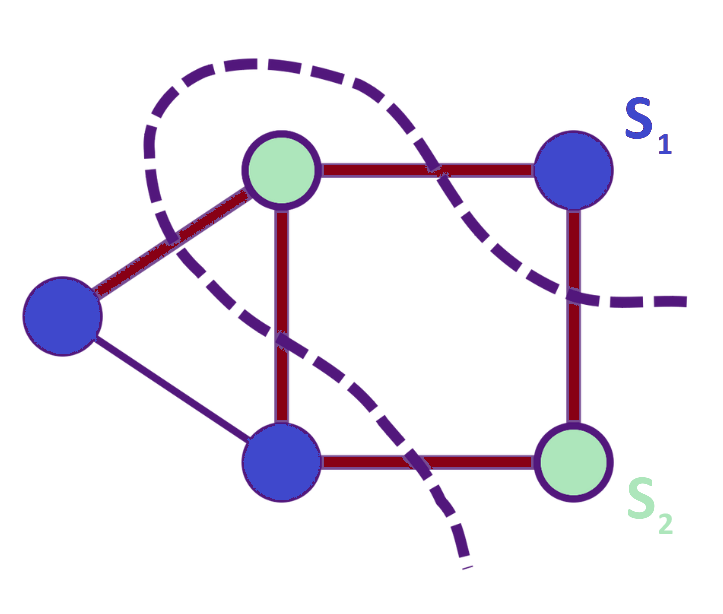
\includegraphics[width=0.95\columnwidth]{Figures/MaxCut.png}
  \caption{An example of a graph with a partition that maximizes the number of cut edges (red). Note that the MaxCut partition might not be unique.} % 'The number of edges that are cut is promptly labeled as the "cut".' Removed!
  \label{fig:MaxCut}
\end{figure}

\subsection{State-of-the-Art Algorithms}
\label{sec: SoA}
Next, we introduce the state-of-the-art algorithms for tackling the MaxCut problem, encompassing both classical (Goemans-Williamson) and hybrid quantum-classical (QAOA and QEMC) approaches.

% QAOA Ansatz image. It's here because of the weird rules that govern figure positioning in LaTeX.
\begin{figure*}[b]
  \centering
  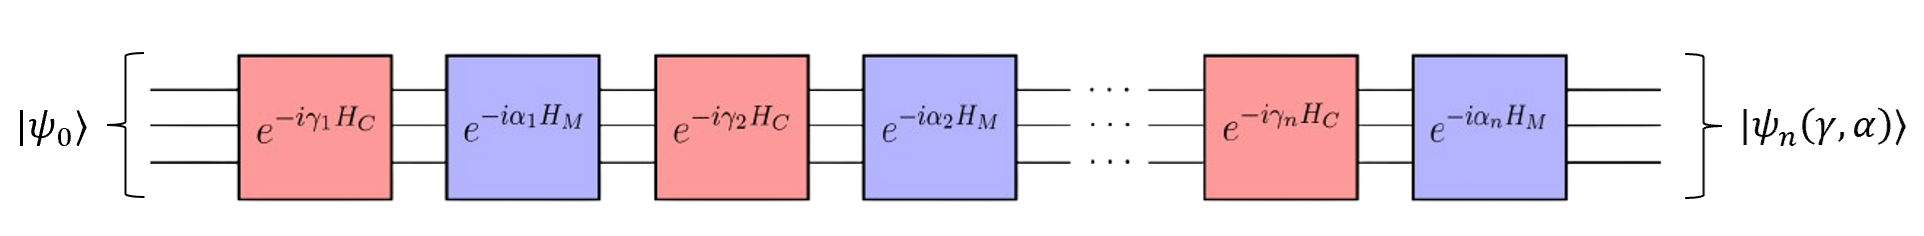
\includegraphics[width = \textwidth]{Figures/QAOA_Trotterization.png}
  \caption{Quantum alternating operator ansatz. Adapted from \cite{Intro_QAOA}.}
  \label{fig:QAOA_Trotterization}
\end{figure*}

\subsubsection{Goemans-Williamson Algorithm}
\label{sec: GW}
%In this section, we explore the Goemans-Williamson (GW) Algorithm, pivotal in combinatorial optimization, especially for MaxCut.

Developed by Goemans and Williamson in 1995, this algorithm employs semidefinite programming to create an approximate solution, later refined for a near-optimal cut. Semidefinite programming optimizes a linear function over a symmetric matrix while ensuring positive semidefiniteness. It finds applications in control theory, nonlinear programming, geometry, and combinatorial optimization, as detailed in \cite{GW-Algorithm} and references therein.

% This can be removed too: "It finds applications in control theory, nonlinear programming, geometry, and combinatorial optimization, as detailed in \cite{GW-Algorithm} and related references."

The Goemans-Williamson algorithm addresses the MaxCut problem through a series of mathematical formulations and randomized procedures. Initially, an integer quadratic program \( (Q) \) is defined to maximize the "cut" in a graph. This is represented by binary variables \( y_i \), where \( S_1 \) and \( S_2 \) correspond to the vertices with values $1$ and $-1$, respectively. However, since solving \( (Q) \) directly is NP-hard, the algorithm instead employs a semidefinite programming relaxation \( (P) \), which relaxes constraints to optimize vectors \( v_i \in S_n \) rather than \( y_i \). This relaxation is represented as:
\begin{equation}\tag{5}
    \begin{aligned}
        &\text{Maximize}\;\;\frac{1}{2}\sum_{\substack{i < j: \\ (i,j)\in E}}(1-v_{i} \cdot v_{j}) \\
        (P)\qquad&\text{Subject to: }v_{i}\in S_n \qquad\forall i\in V,
    \end{aligned}
\end{equation}
where \( v_i \) are vectors constrained to the \( n \)-dimensional unit sphere ($S_n$). The algorithm then proceeds as follows:
\begin{enumerate}
    \item Solve \( (P) \) to obtain optimal vectors \( v_i \);
    \item Select a random vector \( r \) uniformly distributed on $S_n$;
    \item Partition vertices into \( S_1 \) and \( S_2 \) based on whether \( v_i \cdot r \geq 0 \) or \( v_i \cdot r < 0 \).
\end{enumerate}
Effectively, the algorithm divides vertices based on a randomly chosen hyperplane in \( n \) dimensions. The performance guarantee of the Goemans-Williamson algorithm is quantified by the approximation ratio \( \alpha > 0.878 \) \cite{GW-Algorithm}.

%%%%%%%% Separating the two options %%%%%%%%
%%%%%%% This is what I had written before: %
%%% Now, I've cut it short, to have more %%%
%%%%%% space for the other sections. %%%%%%%

% Formally, the Goemans-Williamson algorithm can be described as follows \cite{GW-Algorithm}. Given a graph with vertex set \( V = \{1, ..., n\} \) and non-negative weights \( w_{ij} = w_{ji} \) for each pair of vertices \( i \) and \( j \), the weight of the maximum cut \( w(S_1, S_2) \) is obtained from the integer quadratic program:
% I wonder if I should mention that this formulation is entirely equivalent to the previous expression, with \Chi. If I have space, at the end of this, I guess I can add this.
% \begin{equation}
%     \begin{aligned}\label{eq:GW_Q}
%       &\text{Maximize}\;\;\frac{1}{2}\sum_{\substack{i < j: \\ (i,j)\in E}}w_{i j}(1-y_{i}y_{j}) \\
%       (Q)\qquad&\text{Subject to: }y_{i}\in\{-1,1\}\qquad\forall i\in V,
%     \end{aligned}
% \end{equation}
% where \( S_1 = \{i \mid y_i = 1\} \) and \( S_2 = \{i \mid y_i = -1\} \) correspond to a cut of weight
% \begin{equation}
% w(S_1, S_2) = \frac{1}{2} \sum_{\substack{i < j \\ (i,j) \in E}} w_{ij} \left(1 - y_i y_j\right).
% \end{equation}
% Solving this NP-hard program with the GW algorithm involves relaxing constraints, resulting in a semidefinite programming relaxation \((P)\):
% \begin{equation}
%     \begin{aligned}
%       &\text{Maximize}\;\;\frac{1}{2}\sum_{\substack{i < j: \\ (i,j)\in E}}w_{i j}(1-v_{i} \cdot v_{j}) \\
%       (P)\qquad&\text{Subject to: }v_{i}\in S_n \qquad\forall i\in V.
%     \end{aligned}
%     \end{equation}    
% The GW algorithm then proceeds as follows:
% \begin{enumerate}
%   \item Solve \((P)\) to obtain optimal vectors \( v_{i} \);
%   \item Select a random vector \( r \) uniformly distributed on \( S_n \) ($n$-dimensional unit sphere);
%   \item Partition vertices into \( S_1 \) and \( S_2 \) based on whether \( v_{i} \cdot r \geq 0 \) or \( v_{i} \cdot r < 0 \).
% \end{enumerate}
% This method essentially partitions vertices based on a randomly chosen hyperplane in \( n \) dimensions, dividing them into \( S_1 \) and \( S_2 \) accordingly. Furthermore, it can be shown that the GW algorithm has a performance guarantee of:
% \begin{equation}
%   \alpha=\operatorname*{min}_{0\,\leq\,\theta\leq\pi}\,\frac{2}{\pi}\,\frac{\theta}{1\,-\,\cos\,\theta} > \,0.878.
% \end{equation}
% A comprehensive proof outlining the derivation of this $0.878$ value is available in section $3$ of \cite{GW-Algorithm}, along with a more in-depth exposition of the algorithm.

% I should, at some point, say that I present these state-of-the-art algorithms to provide a benchmark for the iQAQE algorithm. This is important to show that the iQAQE algorithm is competitive with the best algorithms available.

\subsubsection{Quantum Approximate Optimization Algorithm (QAOA)}
\label{sec: QAOA}
% In accordance with the previous section, it suffices to present the QAOA cost function and ansatz to fully characterize it.
% Define the cost as the expectation value of the so-called cost/problem Hamiltonian. Present the form of this Hamiltonian and explain why it works (interpretation, essentially).
% Then, present the Trotter-inspired ansatz: the Quantum Alternating Operator Ansatz. Put the image and explain what the blocks means: cost/problem Hamiltonian and mixer/bias Hamiltonians' complex exponentials. Present these Hamiltonians' forms and their complex exponentials' circuit implementation.
% Also, mention that the uniform superposition enters the ansatz, and the partition is decided by the most frequently sampled basis state, at the end of the circuit, after training.

The QAOA, renowned for its prowess in quantum-enhanced optimization, was initially crafted to tackle a range of combinatorial optimization problems such as constraint-satisfaction \cite{lin2016performance} and MaxCut \cite{PhysRevA.97.022304}. QAOA utilizes a cost Hamiltonian, denoted as \(H_C\), which serves as the basis for extracting the objective function. This Hamiltonian is formed by associating each conventional classical variable $y_i$ with a Pauli spin \(1/2\) operator, represented as \(\boldsymbol{Z}_j\). Formally, the usual MaxCut objective $L(y) = \frac{1}{2}\sum_{\substack{i < j: \\ (i,j)\in E}}(1-y_{i}y_{j})$, denoting the cut of partition $y = (y_1,...,y_N)$, is transformed into the cost Hamiltonian
\begin{equation}\label{eq:H_C}\tag{6}
  H_C = \frac{1}{2}\sum_{\stackrel{i < j:}{(i,j)\in E}}(1-\boldsymbol{Z}_i\boldsymbol{Z}_j).
\end{equation}

The Trotter-inspired QAOA ansatz involves $n$ cycles of alternating time evolution between $H_C$ and a mixer Hamiltonian, $H_M = \sum_{j=1}^{N} \boldsymbol{X_j}$, for $N$ qubits and graph nodes. The role of this mixer Hamiltonian can be understood as introducing quantum fluctuations, or transitions, between different states, helping the algorithm explore the solution space more effectively, ideally preventing it from getting trapped in sub-optimal local minima. This ansatz, depicted in Figure \ref{fig:QAOA_Trotterization}, illustrates $n$ QAOA layers, each comprising alternating applications of $H_C$ and $H_M$. 

The cost function \(C(\boldsymbol{\gamma}, \boldsymbol{\alpha})\) is determined by the expectation value of \(H_C\) over the ansatz state \(\ket{\psi_n(\boldsymbol{\gamma}, \boldsymbol{\alpha})}\), obtained at the end of the quantum circuit (Figure \ref{fig:QAOA_Trotterization}). In practice, defining $\boldsymbol{\theta} = \{\boldsymbol{\gamma}, \boldsymbol{\alpha}\}$, the cost function is $C(\boldsymbol{\gamma}, \boldsymbol{\alpha}) = \bra{\psi_n(\boldsymbol{\gamma}, \boldsymbol{\alpha})}H_C\ket{\psi_n(\boldsymbol{\gamma}, \boldsymbol{\alpha})}$, with
\begin{equation}\label{eq:QAOA_ansatz}\tag{7}
    \scalebox{0.825}{$\displaystyle
    \ket{\psi_n(\boldsymbol{\gamma}, \boldsymbol{\alpha})} = e^{-i\alpha_nH_M}e^{-i\gamma_nH_C} ... e^{-i\alpha_1H_M}e^{-i\gamma_1H_C}\ket{\psi_0},$}
\end{equation}
where $\ket{\psi_0}$ is the initial state entering the ansatz. In QAOA, it is customary to start with a uniform superposition over the $N$ bit-string\footnote{Keep in mind, there's one qubit allocated for each graph node.} basis states, i.e., $\ket{\psi_0} = \ket{+}^{\otimes N}=\frac{1}{\sqrt{2^{N}}}\sum_{z\in\{0,1\}^{N}}\ket{z}$. This is achieved by applying a Hadamard gate to each of the qubits, at the start of the quantum circuit.

In practice, the mixer Hamiltonian terms $e^{-i\alpha_l H_M}$ correspond to $R_x(2\alpha_l)$ and are easy to implement. The cost Hamiltonian terms, on the other hand, are a bit more tricky, requiring the use of $2$ CNOT gates. Each of the terms $e^{-i\gamma_l(1-\boldsymbol{Z}_{j}\boldsymbol{Z}_{k})/2}$ can be transpiled into a quantum circuit, as shown in Figure \ref{fig:Z_iZ_jDecomposition}. For each edge in the graph, we'll have one of these terms, in each of the $n$ layers of the QAOA ansatz.
\begin{figure}[H]
  \centering
  \begin{quantikz}
  \lstick{Qubit $i$} & \ctrl{1} & \qw                & \ctrl{1}  & \qw & \\
  \lstick{Qubit $j$} & \targ{}  & \gate{R_z(\gamma_l)} & \targ{}   & \qw & \\
  \end{quantikz}
  \caption{$e^{i\gamma_l \boldsymbol{Z}_{i} \boldsymbol{Z}_{j} /2}$ decomposition.}\label{fig:Z_iZ_jDecomposition}
\end{figure}

Subsequently, a classical routine is employed to optimize the values of the parameters by minimizing the negative of the cost (analogous to the "cut"), therefore enabling the extraction of the MaxCut partition.

\begin{figure*}[b]
  \centering
  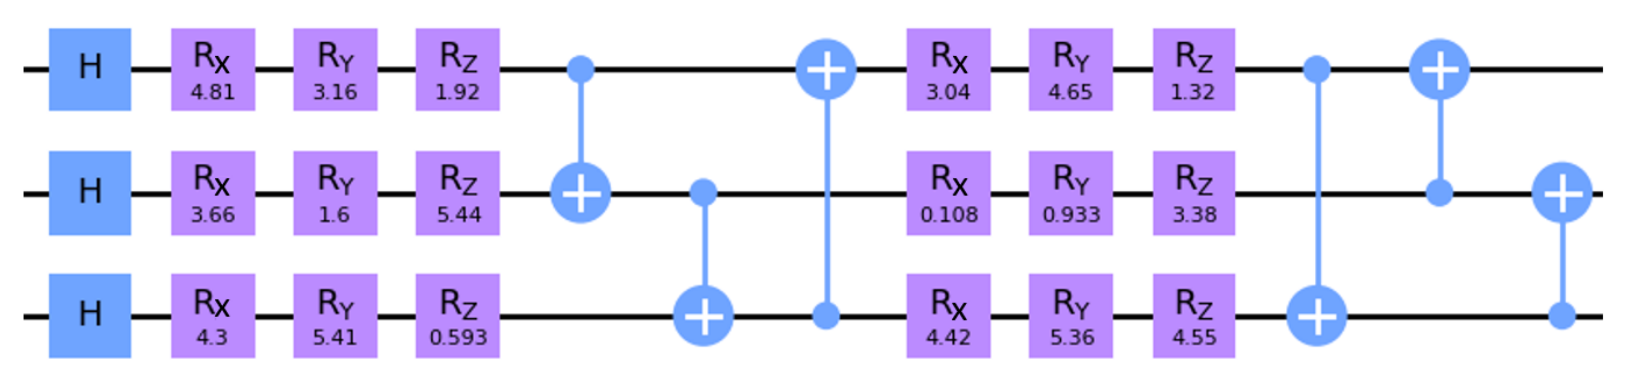
\includegraphics[width = \textwidth]{Figures/Strongly_Entangling_Layers.png}
  \caption{"Strongly Entangling Layers" circuit ansatz: case of $n = 3$ qubits and $p = 2$ layers. After a single layer of Hadamard gates, each subsequent layer consists of $3n$ single-qubit parameterized rotation gates and $n$ CNOT gates (entangling gates). Reproduced from \cite{tenecohen2023variational}.}
  \label{fig:Strongly_Entangling_Layers}
\end{figure*}

\subsubsection{Qubit-Efficient MaxCut Heuristic Algorithm (QEMC)}
\label{sec: QEMC}
% Just summarize the thesis's section on this.

QEMC \cite{tenecohen2023variational} is somewhat similar to QAOA. However, it has a number of crucial differences. First, it only requires $n = \log_2(N)$ qubits, instead of $N$, where $N$ is the number of nodes in the graph. Additionally, the QEMC algorithm is based on a novel probability threshold encoding scheme, a suitable cost function, and a parameterized unconstrained quantum circuit. Going in order: \vspace{1.5mm}

\noindent {\bf \myFontSize Probability threshold encoding scheme:} With $n$ qubits, each of the $N = 2^{n}$ basis states will represent one of the graph's nodes. Following the sampling of the quantum circuit, a probability distribution is generated. Nodes with probabilities exceeding a certain threshold, $p_{th} = \frac{1}{2B}$, belong to "Set 1", while probabilities below this value indicate inclusion in "Set 0". This strongly diverges from how we encode set inclusion in QAOA. \\

\noindent {\bf \myFontSize Cost function:} The objective function utilized in QEMC is the following:

\begin{equation}\tag{8}
    \scalebox{0.75}{$\displaystyle
    L(\{p(i)\}) = \sum_{\stackrel{j < k:}{(j,k)\in E}}\left[\left(d(j,k)-\frac{1}{B}\right)^{2}+\left(s(j,k)-\frac{1}{B}\right)^{2}\right],$}
\end{equation}
where $d(j,k) = |p(j) - p(k)|$ and $s(j, k) = p(j) + p(k)$ are the absolute difference and sum of the corresponding states' probabilities. The idea is that as both $d(j, k)$ and $s(j, k)$ tend towards $1/B$, the probability of one node approaches zero (distinctive "Set 0"), while the probability of the other node approaches $1/B$ (distinctive "Set 1"), without specifying which is which. Ultimately, just like for QAOA, connections between nodes of different sets are favoured. Note, however, that this probability threshold encoding scheme assumes \textit{a priori} that one of the sets ("Set 1") has $B$ nodes. Nevertheless, this is not an issue, as we can efficiently iterate through all potential values of $B\,=\,1,...,\left\lfloor{\frac{N}{2}}\right\rfloor$. Frequently, it is reasonable to set $B = N/2$, and we shall use this as our default starting point. \\

\noindent {\bf \myFontSize Problem-agnostic ansatz:} The QEMC circuit ansatz is agnostic to specific graph instances, a departure from QAOA where the graph structure is explicitly encoded in the quantum circuit. Instead, the graph is implicitly encoded through the cost function. As a result, the QEMC quantum circuit is not bound to any particular form and only needs to be expressive enough to approximate the optimal states in the Hilbert space. Such problem-independent ansatz approach provides considerable flexibility in ansatz selection. Frequently, the circuit ansatz known as "Strongly Entangling Layers" is employed, as depicted in Figure \ref{fig:Strongly_Entangling_Layers}. As can be seen, this ansatz applies a series of parameterized single-qubit rotations interspersed with entangling gates to generate a highly entangled quantum state. % We use PennyLane's \href{https://docs.pennylane.ai/en/stable/code/api/pennylane.StronglyEntanglingLayers.html}{\texttt{qml.StronglyEntanglingLayers}} implementation for this purpose.

% Can, maybe, remove "As can be seen, this ansatz applies a series of parameterized single-qubit rotations interspersed with controlled entangling gates to generate a highly entangled quantum state. We use PennyLane's \href{https://docs.pennylane.ai/en/stable/code/api/pennylane.StronglyEntanglingLayers.html}{\texttt{qml.StronglyEntanglingLayers}} implementation for this purpose."

% These constitute the main ingredients necessary to understand the QEMC algorithm. At this point, the same hybrid loop as before would be run, so as to optimize the "Strongly Entangling Layers" ansatz's parameters, to minimize the cost function. To read the MaxCut partition, generated by the QEMC algorithm, one would sample the circuit's output one more time, after the training, and build the basis states' probability distribution. The threshold $p_{th}$ would then be applied to determine each nodes' set inclusion, from each of their associated basis states' probabilities.

One notable, and perhaps unfortunate, property of QEMC is that it is efficiently simulable classically. Due to the exponential compression of the number of qubits, the algorithm can be feasibly simulated on a classical computer, even for large graphs, hence defeating its purpose as a quantum algorithm. This is something the authors of the algorithm \cite{tenecohen2023variational} realized in hindsight. For this reason, it is now termed a quantum-inspired classical algorithm.

% For the iQAQE Framework, maybe present the Table?


	\section{iQAQE Framework}
\label{sec: Methodology}

We introduce a new framework, inspired by QAOA and QEMC, for seamlessly designing multiple distinct VQAs. This framework builds on QEMC's core components while integrating concepts from QAOA to leverage the strengths of both algorithms for improved performance. Tentatively named the iQAQE Framework, it opens the door to numerous unexplored and unknown VQAs, offering a variety of parameters to experiment with, such as the number of qubits, list cardinality, and mappings.

In iQAQE, we depart from the QEMC approach by associating each graph node with a list of basis states, in contrast to QEMC's consideration of a single basis state for each node. Each of these lists comprises $c \in \left[1, 2^{n-1}\right]$ basis states, where $n$ represents the number of qubits. $c$ denotes the cardinality of the lists. What we formerly referred to as "mapping" involves distributing basis states among these lists. The term "mapping" can also signify a specific allocation of basis states among the lists. This design allows for potential overlap among states from different lists. Additionally, it is important to note that the encoding of these states will utilize a qubit range expected to fall between the QEMC and QAOA requirements, specifically in $[\log_2{N}, N]$, for an $N$-node graph.

As a default approach, we compute node probabilities straightforwardly by summing the probabilities of associated basis states and then normalizing the result. This is necessary because we utilize QEMC's probability threshold encoding scheme. Additionally, we consider iQAQE to use the same ansatz and cost function as QEMC, adjusted for the appropriate number of qubits. However, we also explore the potential for slight deviations from this formula, such as alternative methods for computing node probabilities and the adoption of problem-inspired ansatz variations.

We can postulate that such a hybrid approach might have some potential advantages. Namely, it should allow for less shots than in QEMC and fewer qubit requirements than in QAOA, in addition to, arguably, being better trainable \cite{tenecohen2023variational}. Another notable feature of this algorithm is its tunable "quantum-ness." By interpolating between QAOA (a hybrid quantum-classical method) and QEMC (a classical, quantum-inspired method), we can selectively adjust the degree of quantum and classical components, which could prove to be advantageous.

We designate this as a framework due to the vast array of possibilities in qubit number, list cardinality, and mappings, which facilitate the creation of multiple unique VQAs, each with its own merits and drawbacks. In this study, we will present heuristics for parameter selection and provide a comprehensive analysis of the corresponding results.

% Maybe, I should explain why we believe this should yield better results. Less qubits, shallower circuits, tunable "quantum-ness", etc.

% The primary objective of this study is to ascertain the optimal mapping from basis states to lists, essentially determining which basis states should be included in specific lists/nodes. Naturally, this undertaking also involves the identification of a suitable cost function and ansatz to ensure the algorithm's effective operation. For most of our work, we consider iQAQE to use the same ansatz and cost function as QEMC, adjusted for the appropriate number of qubits and with some modifications that we'll discuss below.
	\section{Implementation}
\label{sec:resul}

In our numerical implementation, we leveraged PennyLane, a Python library tailored for differentiable programming of quantum computers. PennyLane facilitates the execution of variational quantum circuits and their simultaneous training, akin to training a classical neural network, within the same Python environment. We utilized two PennyLane devices: \texttt{default.qubit} for smaller circuits and exact expectation values, and \texttt{lightning.qubit} for larger circuits. Furthermore, NetworkX was instrumental in generating and manipulating graphs for addressing the MaxCut problem, while CVXPY, tailored for convex optimization, assisted in solving the semidefinite programming relaxation of MaxCut within the Goemans–Williamson algorithm framework.

Despite the versatility of our setup, testing on actual quantum hardware was unavailable, limiting our evaluation to simulations on a personal computer. This constraint also impacted scalability and comprehensive testing, particularly for larger graphs. Simulations were conducted using the Adam optimizer, with learning rates fine-tuned as hyperparameters.

% Maybe swap the order of the following two paragraphs.
Moreover, it's important to elucidate the methodologies employed for benchmarking and testing the algorithms' efficacy. Central to our evaluation are the cost and approximation ratio\footnote{The approximation ratio denotes the proportion of the achieved "cut" value to the MaxCut value.} plots, essential for comparing convergence rates and final cut values across the algorithms. Additionally, recognizing the influence of initial parameters on outcomes, we adopt statistically robust metrics such as average cut values and the best-so-far (BSF) cut value, obtained through a monotonic transformation\footnote{If a dip occurs in the graph, it is adjusted to match the previous graph value, ensuring that the final result is monotonically increasing. That's what the BSF transformation does.}. Furthermore, to mitigate the impact of outliers, we incorporate the median BSF cut value in our analysis, computed from multiple training curves to ensure statistical robustness. Frequently, we use the average cut or approximation ratio curves generated from $10$ different random initializations. This approach enables us to evaluate the algorithm's performance on average post-training. Essentially, we assess the likelihood of obtaining favorable results following a single run.

% Maybe swap the order of this paragraph with the previous one.
In our pursuit of optimization, grid searches are conducted on hyperparameters like Adam's learning rate, the number of layers (\texttt{n\_layers}), and qubits (\texttt{n\_qubits}), albeit constrained by the unavailability of an HPC cluster. We also refine our evaluations by benchmarking against the Goemans-Williamson algorithm, offering insights into the relative performance of our algorithms compared to state-of-the-art solutions. Additionally, we extend our comparative analysis to include commonly used quantum optimization algorithms such as QAOA and QEMC. Through these multifaceted evaluations, we aim to provide nuanced insights into the strengths and limitations of each algorithm under consideration.
	\section{iQAQE Schemes and Results}
\label{sec:concl}

% Maybe re-read what I have until here, before resuming writing.

Now, we present the various iQAQE schemes we have developed and the results of their numerical simulations. For a more detailed discussion, please refer to the full thesis (Chapter 5). Keep in mind that all numerical results refer to the same $8$-node graph: \texttt{\myurl{E = [(0, 1), (0, 2), (0, 6), (1, 2), (1, 6), (3, 2), (3, 4), (3, 5), (4, 5), (4, 7), (5, 7), (6, 7)]}}.


% \begin{figure}[t]
%     \centering
%     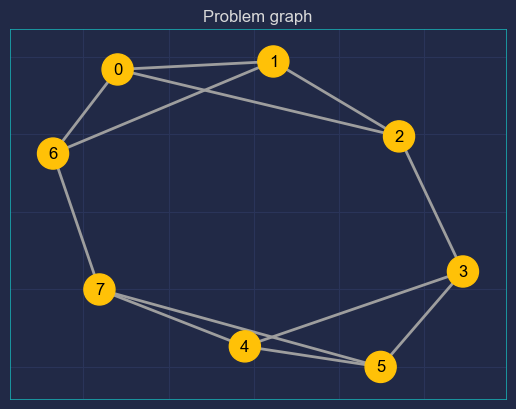
\includegraphics[width=0.95\columnwidth]{Figures/problem_graph.png}
%     \caption{Considered $8$-node graph instance. The optimal cut ($10$) was found through
%     brute-force (exhaustive search).}
%     \label{fig:8_node_graph}
% \end{figure}

\subsection{Random iQAQE}
\label{subsec:Random_iQAQE}

First and foremost, we aim to understand how iQAQE compares with both QAOA and QEMC. For this comparison, $n$ and $c$ were randomly chosen ($n = c = 4$). Currently, the allocation of basis states to lists is also done randomly. The goal of this initial simulation is to take a preliminary look at iQAQE's performance and understand how much the results vary between finite shot number simulations and analytical ones (Figure \ref{fig:3_Comparison_shots}). These plots generally align with our theoretical expectations. As QEMC relies heavily on a large number of shots, transitioning to a finite shot number naturally impacts the results. Surprisingly, however, iQAQE seems to exhibit slightly greater resilience to this effect, despite sharing QEMC's cost function and ansatz. This resilience might be attributed to the presence of multiple basis states associated with each graph node, potentially reducing the need for exhaustive sampling.

% Chapter 5's figure. Positioning!
\begin{figure*}[t]
    \centering
    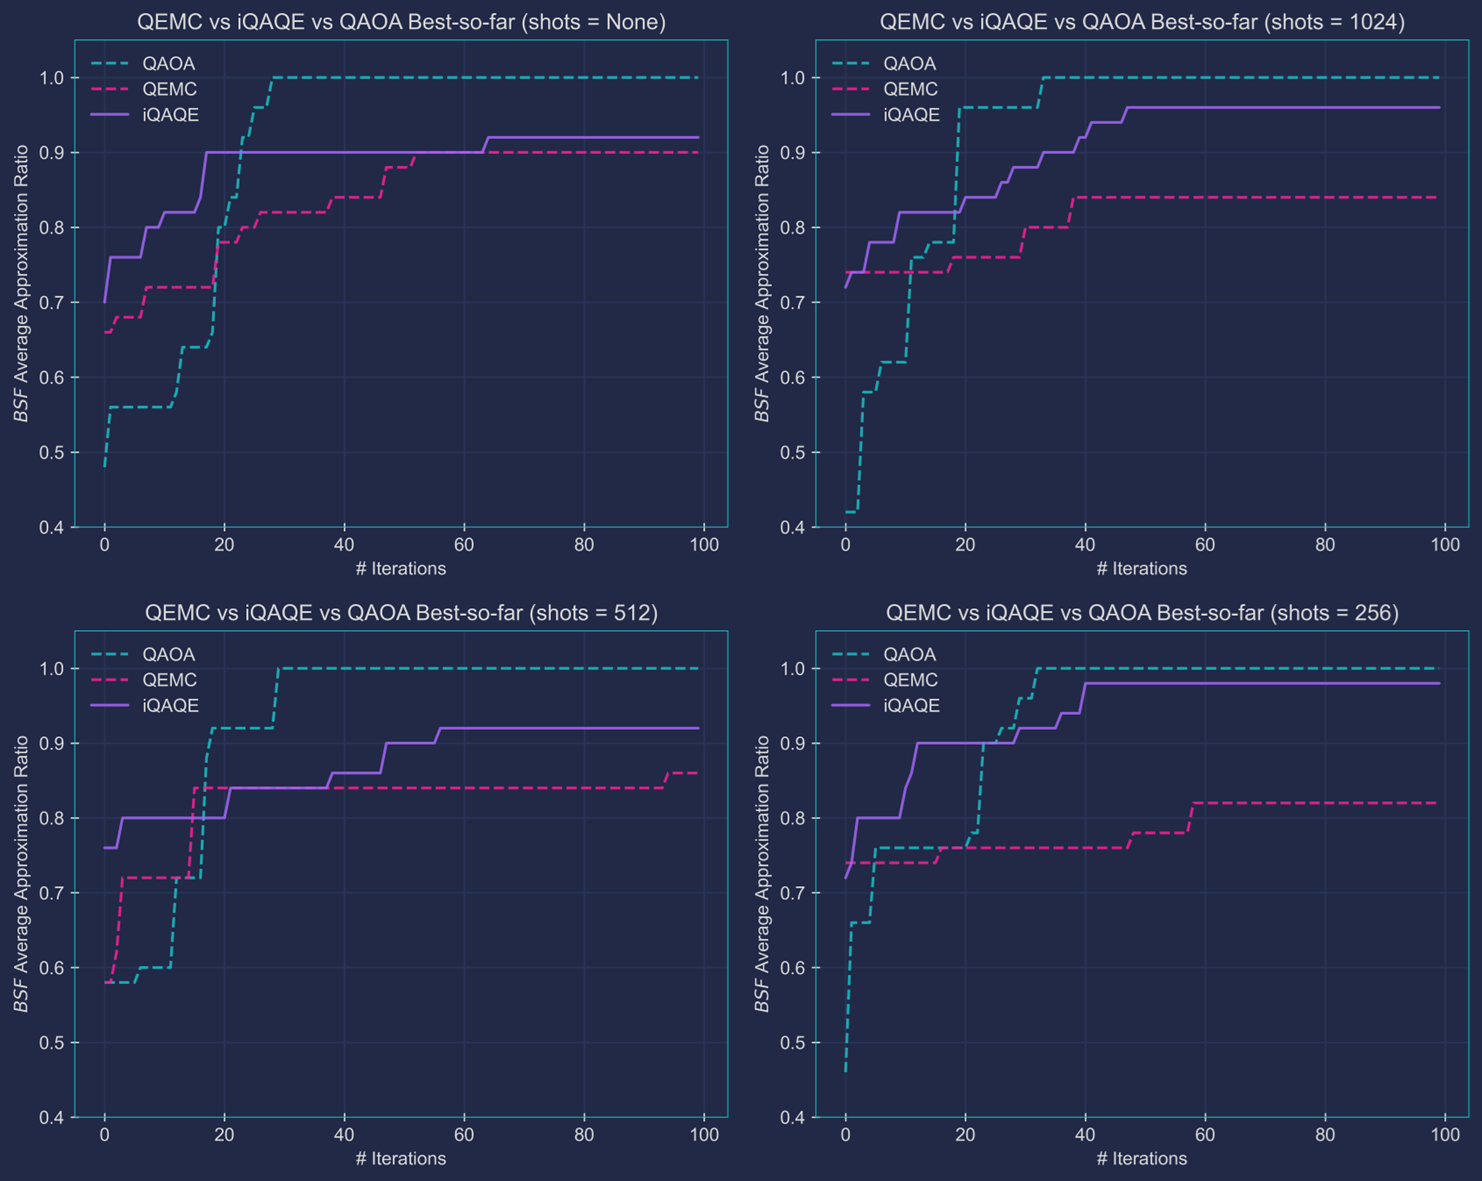
\includegraphics[width=0.90\textwidth]{Figures/Random_iQAQE_Updated.png}
    \caption{Comparison between the $3$ VQAs' performances (QAOA, QEMC and iQAQE), using an infinite and finite number of shots. The best-so-far average is plotted ($8$-node graph).}
    \label{fig:3_Comparison_shots}
\end{figure*}

\subsection{Polynomial Compression-type Encodings}
\label{subsection:Polynomial_Encodings}
These schemes fix one or more qubits to $1$ (or $0$) while letting the others vary\footnote{Fixing qubits means we only permit basis states where certain qubits are set to either $0$ or $1$. Each node has specific qubits fixed, and these fixed qubits differ between nodes, forming the basis for our mappings.}. Fixing $k$ qubits achieves polynomial compression of order $k$. The total number of nodes encoded is $\binom{n}{k}$, the number of ways to select $k$ qubits from $n$. We select the smallest $n$ such that $\binom{n}{k} \geq N$, resulting in $N = \mathcal{O}(n^k)$. We then decide how many basis states to use for each node, chosen from $2^{n-k}$. We may use all $2^{n-k}$ states or choose a subset $c \leq 2^{n-k}$. Upon selecting the mapping, the algorithm uses QEMC's cost function and ansatz. Polynomial compression ensures $n < N$ unless $k = 1$.

\subsubsection{Basic Polynomial Compression-type iQAQE}
\label{subsubsection:Basic_Polynomial_iQAQE}
\vspace{-2.5mm}
\begin{figure}[H]
    \centering
    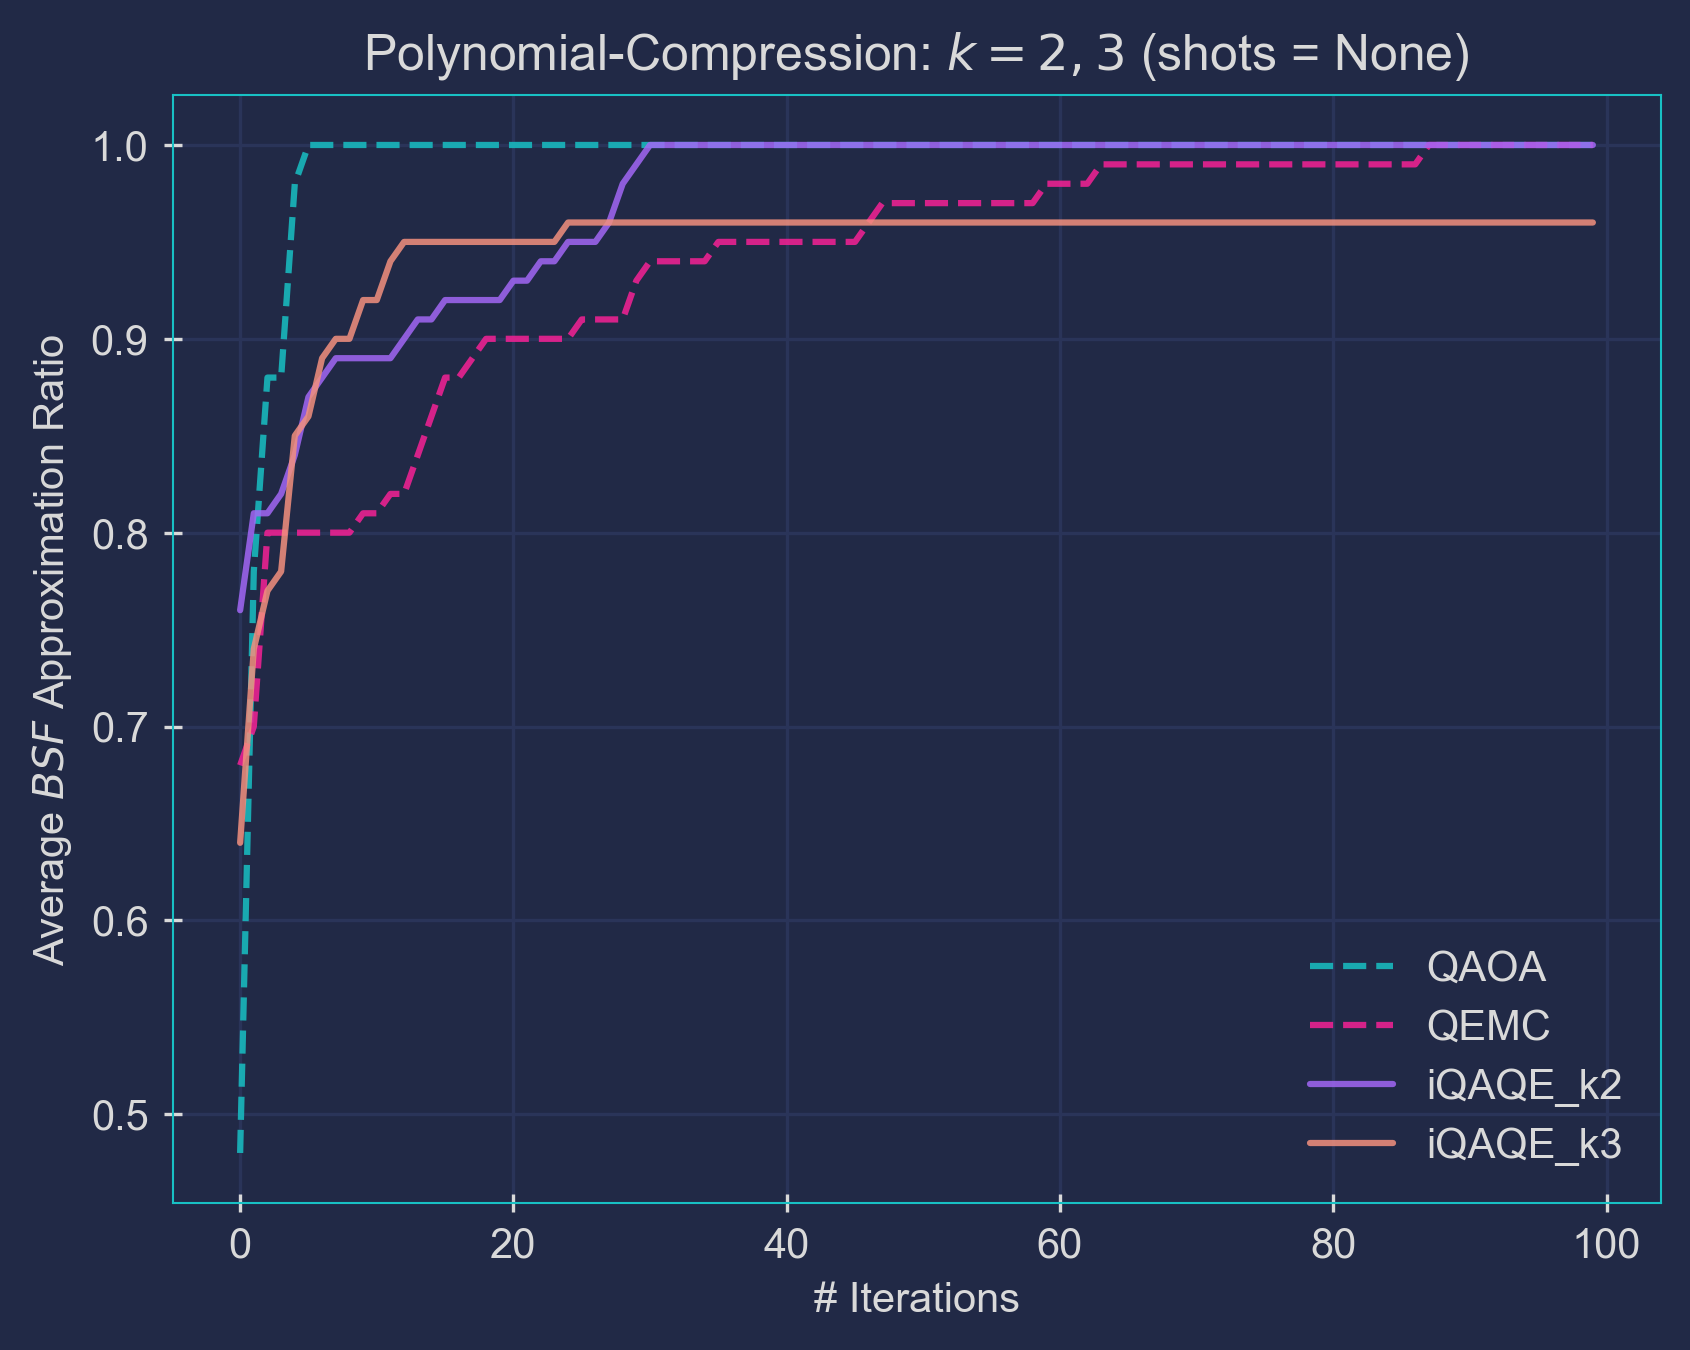
\includegraphics[width=0.95\columnwidth]{Figures/Polynomial_Compression_Base_k2_k3_1.png}
    \caption{Average BSF Approximation Ratio \textit{vs.} iteration number for the tested VQAs. The number of layers considered were $4$ for $k = 2$ and $5$ for $k = 3$ ($8$-node graph).}
    \label{fig:Comparison_k2+k3_2}
\end{figure}
\vspace{-3.5mm}
This is the simplest type of polynomial compression-based iQAQE scheme. It involves fixing $k$ qubits to $1$ instead of $0$ (e.g., $\{\ket{11\text{xxx}}\}$, for $k = 2$). The number of fixed qubits ($k$) is determined by the desired order of compression, as previously described. The results for $k = 2$ and $k = 3$ are shown in Figure \ref{fig:Comparison_k2+k3_2}. Results-wise, \texttt{iQAQE\_k2} achieves a perfect average BSF approximation ratio, although it requires more iterations than QAOA. Our method outperforms QEMC for $k = 2$, but yields less promising results for $k = 3$. Nevertheless, both mappings use fewer qubits ($n = 5$) compared to QAOA ($n = 8$), which is advantageous for implementation on practical (NISQ) quantum computers.

\subsubsection{Correlation-based iQAQE}
\label{subsubsection:Correlation_iQAQE}

This scheme closely resembles what was previously discussed in subsection \ref{subsubsection:Basic_Polynomial_iQAQE}. The key distinction lies in the inclusion of the possibility for both $0$'s and $1$'s to be fixed (e.g., $\{\ket{11\text{xxx}}, \ket{00\text{xxx}}\}$, for $k = 2$; recall, this encodes a single node). Consequently, the scheme aims to identify correlations among the different qubits, wherein "correlations" denote identical colors. This approach was inspired by the notion that by identifying correlations between nodes, it becomes feasible to color the entire graph as long as one node is initially colored. We present the results of numerical simulations applied to the standard $8$-node graph using this correlation-based iQAQE approach (Figure \ref{fig:Correlation/k=2,3,4}).

% Removed!
% In other words, the constructed lists regard the $k$ fixed qubits as positively correlated, meaning they are either all set to $1$ or all set to $0$.

% Also removed!
% Although seeking correlations between qubits, as done here, differs from seeking correlations between nodes, we anticipated that it might yield promising results to some extent. In this scenario, the color of each node is determined by the probability that its $k$ associated qubits are all positively correlated.

\begin{figure}[H]
    \centering
    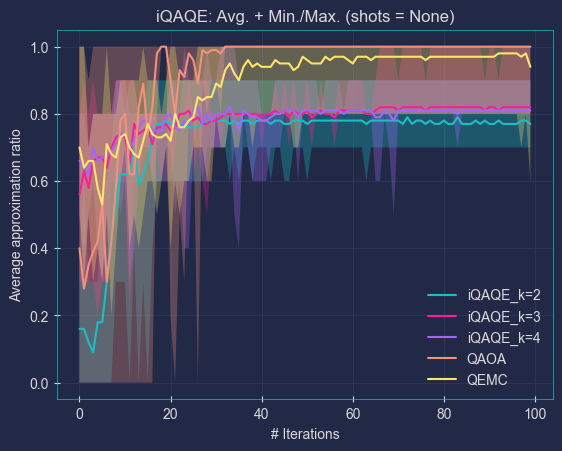
\includegraphics[width=0.95\columnwidth]{Figures/Correlation-based/k=2_3_4.png}
    \caption{Comparison of correlation-based iQAQE results for $k=2, 3$, and $4$ with outcomes from QAOA and QEMC ($8$-node graph).}
    \label{fig:Correlation/k=2,3,4}
\end{figure}

The underperformance may stem from doubling the number of basis states in each sub-list, resulting in a $50\%$ overlap between pairs of sub-lists, akin to Basic Polynomial Compression-type iQAQE. However, this time, with twice the basis states, the (absolute) overlap is significantly higher, leading to more shared states among nodes. When overlap is excessive, adjusting one node's color without affecting others becomes more challenging, likely causing the underperformance.

\subsubsection{Fixed-Parity iQAQE}
\label{subsubsection:Fixed-Parity_iQAQE}

Now, we present another heuristic method for mapping the basis states to the nodes. Although it is similar to the previous one, this time we fixed the parity of the selected $k$ qubits to be even. Parity is determined by the number of $1$'s: if the count is even, the parity is even; otherwise, it is odd. For instance, for $k=3$ (with \texttt{n\_qubits = 5}), the lists would take the form: (Keep in mind that we are using an $8$-node graph.)
% \vspace{-10mm}
% Remeber that 'k=2' is the same as the previous correlation-based! Mention this in the text!
{\normalsize\begin{enumerate}[itemsep=0mm]
    \item $\left\{\ket{000\text{xx}}, \ket{011\text{xx}}, \ket{101\text{xx}}, \ket{110\text{xx}}\right\}$;
    \item $\left\{\ket{00\text{xx}0}, \ket{01\text{xx}1}, \ket{10\text{xx}1}, \ket{11\text{xx}0}\right\}$;
    \item $\left\{\ket{0\text{xx}00}, \ket{0\text{xx}11}, \ket{1\text{xx}01}, \ket{1\text{xx}10}\right\}$;
    \item $\left\{\ket{\text{xx}000}, \ket{\text{xx}011}, \ket{\text{xx}101}, \ket{\text{xx}110}\right\}$, etc.
\end{enumerate}} % \vspace{-10mm}
\noindent We have presented only the first four nodes. Numerical simulations were performed, and the obtained results are presented in Figure \ref{fig:Fixed-parity/k=2,3,4}. While performance still lags behind QAOA, it is notably better than the previous scenario. For $k=2$, the results match the previous correlation-based scheme, as requiring pairs to be even is equivalent to requiring them to be the same.
% \vspace{-10mm}
\begin{figure}[H]
    \centering
    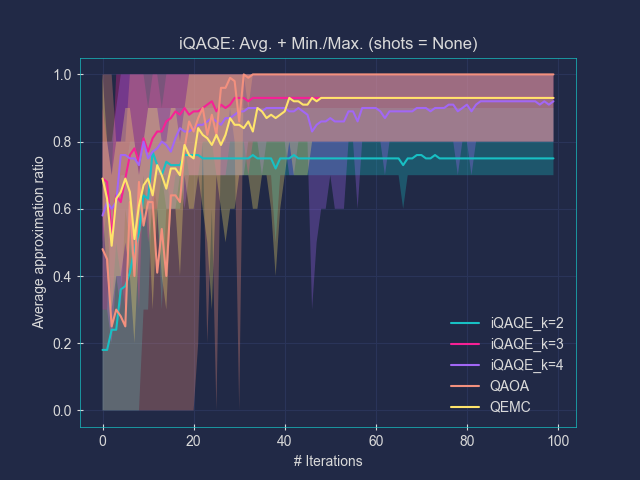
\includegraphics[width=0.95\columnwidth]{Figures/Fixed-parity/k=2_3_4(8-node).png}
    \caption{Fixed-parity iQAQE for $k=2, 3$, and $4$ compared with the results from QAOA and QEMC ($8$-node graph).}
    \label{fig:Fixed-parity/k=2,3,4}
\end{figure}
% \vspace{-10mm}

\subsection{Unmodified Extended-QEMC}
\label{subsection:Vanilla_Extended_QEMC}

\begin{figure}[H]
    \centering
    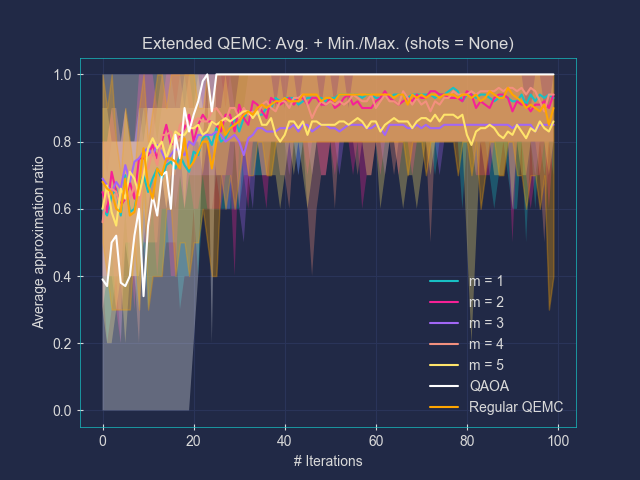
\includegraphics[width=0.95\columnwidth]{Figures/Extended-QEMC/8-node(n_layers=3, step_size=0.95, m=All).png}
    \caption{Implementation of the Unmodified Extended-QEMC scheme for the usual $8$-node graph: comparison with QAOA and regular QEMC for various values of $m$. Note that $m$ is not extended beyond $5$, as this would exceed the number of qubits used in QAOA. Additionally, we utilize \texttt{n\_layers = 3}, \texttt{step\_size = 0.95} and \texttt{B = 4}.}
    \label{fig:Vanilla_Extended-QEMC}
\end{figure}

Amid the various schemes we've attempted, I've devised an extension to the standard QEMC scheme. This new approach enhances QEMC by incorporating $m$ additional qubits beyond the usual $\lceil\log_2(n)\rceil$ qubits required for $n$ graph nodes. This increase in qubits prevents the scheme from being easily classically simulable and allows for more basis states to be associated with each graph node. This scheme assigns $2^m$ basis states per node. Importantly, similar to QEMC, the sets of basis states associated with different nodes do not overlap. The assignment of states to each list is currently arbitrary. For simplicity, we use a straightforward partition: the first $2^m$ basis states go to the first list, the next $2^m$ to the second list, and so on. Now, I present the results of applying this scheme to the usual $8$-node graph (Figure \ref{fig:Vanilla_Extended-QEMC}).

\subsection{Alternative ansätze}
\label{subsection:Alternative_Ansätze}
After considering whether QEMC and iQAQE could be affected by a generic ansatz, I pondered if tailored ansätze and excess entanglement might impact performance. To address this, I proposed implementing non-deterministic CNOT gates (ND-CNOTs\footnote{We recognize that the term "non-deterministic CNOT gates" is employed in linear optical quantum computing (KLM protocol), yet we use it differently in this context.}), adjusting entanglement dynamically. We achieved this by adding parameterized $R_x$ gates before each CNOT's control qubit. Following numerical testing, we discovered that despite increasing complexity in the optimization landscape, this seems to substantially improve performance, especially when coupled to QEMC.

\subsection{Goemans-Williamson and Bigger Graphs}
\label{subsection:GW_Bigger_Graphs}

\begin{figure}[H]
    \centering
    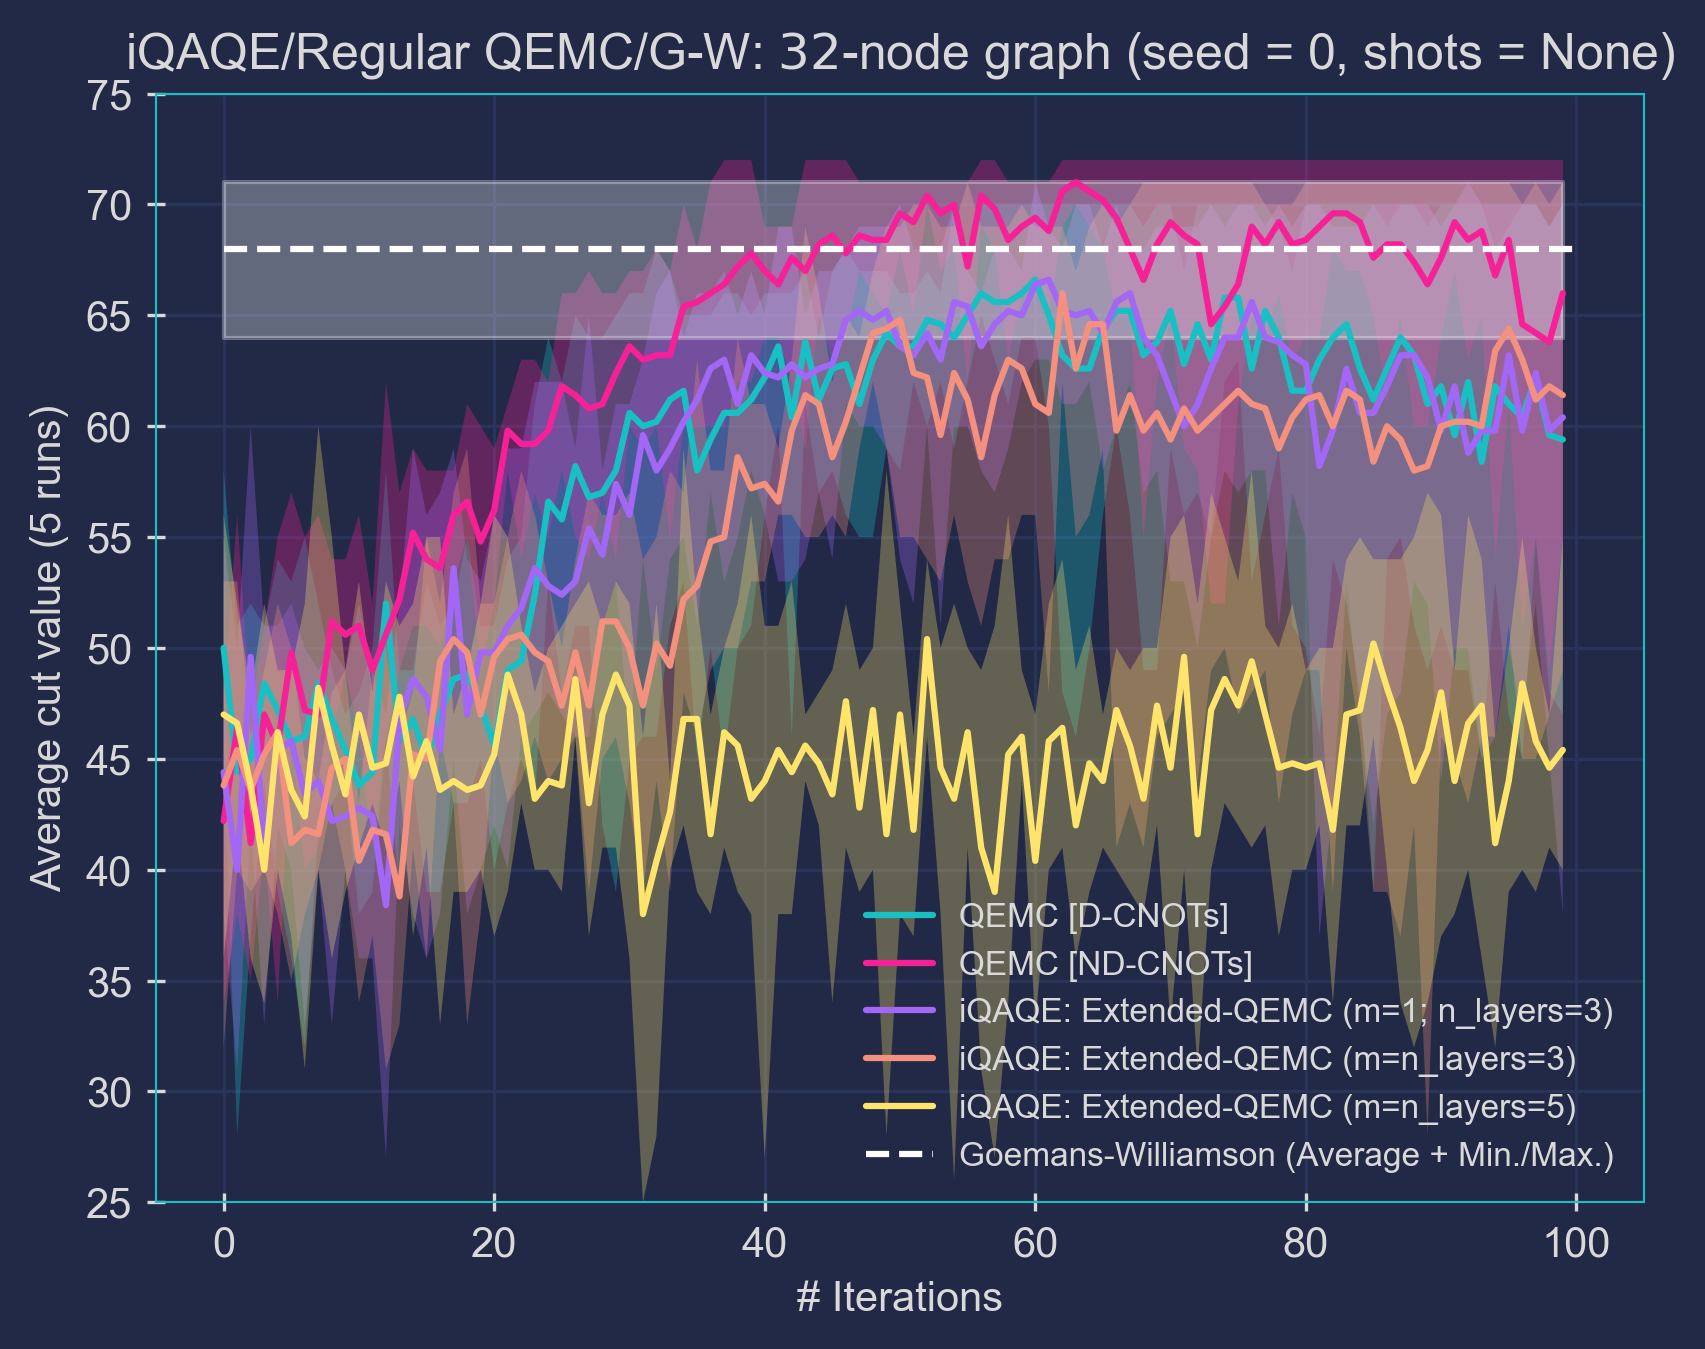
\includegraphics[width=0.95\columnwidth]{Figures/Large graphs/32-node_Graph_seed=0.png}
    \caption{Comparison of performance (average cut values) among various VQAs for a $32$-node graph.}
    \label{fig:32-node_Graph}
\end{figure}

To assess the scalability of these algorithms, we conducted tests on larger graphs, facilitating more accurate comparisons with classical state-of-the-art methods (GW). The results ($32$-node graph) for the most promising algorithms are depicted in Figure \ref{fig:32-node_Graph}. Remarkably, the average performance of ND-CNOT-based QEMC competes closely with GW, occasionally surpassing it. Moreover, the maximum performance of the same ND-CNOT QEMC exceeds that of GW, as seen in Figure \ref{fig:32-node_Graph} (shaded regions). This marks the first instance in our study where one of our heuristics outperforms classical state-of-the-art algorithms, highlighting significant progress and indicating the potential for further exploration within the proposed iQAQE Framework. Other heuristics were explored in this project but are not included here due to space limitations. We have presented the most significant results, though all findings are important and should not be overlooked. For a thorough discussion, please consult the full thesis (Chapter 5).

\subsection{Randomized iQAQE benchmarking -- Machine learning-based approach}
\label{subsection:Randomized_iQAQE_ML}
We also proposed a scheme for determining the optimal mapping for a specific graph based on statistical properties of the mappings themselves, using a small machine learning model. Such a model necessitates defining input (independent variables - IVs) and output (dependent variable - DV). Our IVs will encompass statistically significant properties\footnote{Examples: number of basis states, average Hamming weight, average pair-wise Hamming distance, etc.} extracted from each node's specific sub-list. Alternatively, including the basis states' mapping directly as the model's input presents challenges concerning memory-efficient encoding. Traditional one-hot encoding methods are inadequate due to the vast number of potential basis states available (which scales exponentially with the number of qubits). Additionally, the median BSF cut value after training was selected as the DV. Initially, we utilized a multiple linear regression model. Upon observing significant multicollinearity among some IVs, we transitioned to principal component analysis (PCA), followed by regression (PCR). Although the results were not entirely satisfactory, we believe this approach can inspire future research, building on this idea and our initial work. For a more detailed discussion, please refer to the full thesis (Chapter 5).
	\section{Alternative Schemes}
\label{sec:Alternative_Schemes}

% Maybe I'll remove this section altogether, due to space limitations. I think I'll just briefly mention this somewhere else. Maybe at the end of the previous (iQAQE Schemes and Results) section.

We also developed alternative schemes that, although not entirely based on the iQAQE Framework, emerged from our research on these topics. These are different algorithms proposed to solve the MaxCut problem. Two such alternatives are the Parity-like QAOA and the Batch-based Oracle coloring scheme. The former involves "reducing" QAOA's problem Hamiltonian to use fewer qubits than usual, by using parity encodings, which allow us to compress the representation of \(N\) nodes into \(n < N\) qubits (with \(N = \mathcal{O}(n^k)\), for any \(k\), as long as \(\binom{n}{k} \geq N\)). The latter could be implemented with a trainable Oracle, which would receive $k < n$ qubits, and return the colors of $k$ nodes. Afterwards, we would run $\frac{n}{k}$ batches of this, to obtain all the $n$ nodes' colors. Due to space constraints, we won't discuss these schemes in detail in this extended abstract; we simply present them. For a detailed discussion, please see Chapter 6 of the thesis.
	\section{Conclusions}
\label{sec:Conclusions}
% Results paragraph:
The primary accomplishment of this study is the development of the iQAQE Framework, offering promising competition with current state-of-the-art algorithms. We've showcased its advantages over QAOA and QEMC, particularly in terms of reduced qubit requirements and enhanced resilience to statistical uncertainty. Our introduced heuristics have generally shown competitive results, even surpassing classical state-of-the-art (GW) in certain scenarios, like ND-CNOT-based QEMC for a $32$-node graph. This success underscores the potential of the iQAQE Framework. Moreover, we proposed a method for determining optimal mappings based on statistical properties, utilizing a small machine learning model. While initial results were not entirely satisfactory, we believe this approach can inspire further research.

% Future work paragraph:
Future work could focus on enhancing the machine learning model, developing new heuristics, and testing on larger graphs. Exploring neural networks, alternative input variables, and different heuristics configurations could yield valuable insights. Additionally, testing the framework on real-world quantum computers is essential for assessing its practical viability. Further refinement and testing of proposed heuristics will also be crucial for continued improvement. Another research direction is to further develop the alternative schemes presented in section \ref{sec:Alternative_Schemes}, which could provide valuable insights and potential avenues for future study. By addressing these areas, future research can build upon the foundation laid by this work, potentially leading to significant advancements in VQAs.

% Additionally, testing the framework on real-world quantum computers is essential for assessing its practical viability.
% Think of this as: "The algorithm's performance could be very significantly affected by the hardware's noise, rendering it less effective than expected. Therefore, testing on real-world quantum computers is essential for assessing its practical viability."

\section*{Acknowledgments}
\label{sec:Acknowledgments}
This work was developed in collaboration with Zoltán Zimborás and Bence Bakó, from the Wigner Research Centre for Physics (Hungary), in the context of project: \textit{HQCC – Hybrid Quantum-Classical Computing}, supported by the EU QuantERA ERA-NET Co-fund in Quantum Technologies and by FCT -- Funda\c{c}\~{a}o para a Ci\^{e}ncia e a Tecnologia (QuantERA/004/2021).

% Re-read everything and make sure it's all good. Might remove some parts in the introduction/background to make space for more results.

% Should also re-read my thesis one more time, to make sure I didn't mess anything up, when copying stuff from there to here.

\nocite{Tabi_2020,nielsen2010quantum,sciorilli2024largescale,Karp2010,NP-problems}

% REFERENCES

\begingroup
\footnotesize
% Produces the bibliography section when processed by BibTeX
%
% Bibliography style
% > entries ordered alphabetically
%\bibliographystyle{plain}
% > unsorted with entries appearing in the order in which the citations appear.
% \bibliographystyle{unsrt}
\bibliographystyle{hunsrt}
% > entries ordered alphabetically, with first names and names of journals and months abbreviated
% \bibliographystyle{abbrv}
% > entries ordered alphabetically, with reference markers based on authors' initials and publication year
%\bibliographystyle{alpha}

% External bibliography database file in the BibTeX format (ExtendedAbstract_ref_db.bib)
\bibliography{references}
\endgroup

\end{document}


